\documentclass[10pt]{article}
\usepackage{amsmath,amssymb}
\usepackage{longtable}
\usepackage{tikz}

\usepackage[a4paper,left=2cm,right=2cm,top=1.5cm,bottom=2cm]{geometry}
\usepackage{xcolor}
\setlength{\parindent}{0pt}
\setlength{\emergencystretch}{2em}
\begin{document}

\title{Decision Trees by Hand - Solutions}
\author{}
\date{}
\maketitle
\subsection*{Learning goals}
After this exercise, you should be able to

\begin{itemize}
\item
explain what a regression tree predicts inside a leaf,

\item
explain why the mean is the optimal constant prediction when squared error is used,

\item
interpret residuals, mean squared error (MSE), and sum of squared errors (SSE),

\item
use the mean for squared error and the median for absolute error,

\item
determine all relevant candidate split points for a one-dimensional feature,

\item
reproduce the main steps that a regression-tree training algorithm performs when choosing a split,

\item
construct a shallow regression tree by hand,

\item
explain why a regression tree produces a piecewise-constant prediction,

\item
explain qualitatively how increasing tree depth affects approximation quality and overfitting,

\item
extend the same reasoning to a dataset with more than one input feature,

\item
train trees using absolute error and combine trees fitted to bootstrap samples into a forest,

\item
distinguish training error from prediction error at unobserved input positions.

\end{itemize}
The calculations in this sheet are designed to be done by hand. No programming is required.

\clearpage
\section*{Part I - Understanding a single leaf}
\textbf{\textit{Regression}} means predicting a numerical value. An \textbf{\textit{observation}} is one data point; its \textbf{\textit{features}} are the input values, such as $x$, and its \textbf{\textit{target}} $y$ is the value to be predicted. The \textbf{\textit{training data}} are the observations used to choose the model. A prediction is written $\hat y$, and the fitted function is written $\hat f$.

A \textbf{\textit{regression tree}} divides the input space using a sequence of decisions. A \textbf{\textit{node}} contains the observations that reach a particular stage. The \textbf{\textit{root node}} initially contains all training observations. A \textbf{\textit{split}} divides a parent node into two \textbf{\textit{child nodes}}. An \textbf{\textit{internal node}} makes a split; a \textbf{\textit{leaf}} makes no further split and assigns one constant prediction to every input reaching it.

Throughout this sheet, split rules send $x<t$ to the left child and $x\geq t$ to the right child. The \textbf{\textit{threshold}} $t$ is the boundary used in that decision. We use squared error to train the trees, except when explicitly comparing other losses.

Consider a leaf that contains four target values

\begingroup
\small
\setlength{\tabcolsep}{4pt}
\begin{longtable}{l|l}
observation & target $y_i$ \\
\hline
\endfirsthead
observation & target $y_i$ \\
\hline
\endhead
1 & 2 \\[1.5pt]
2 & 3 \\[1.5pt]
3 & 4 \\[1.5pt]
4 & 7 \\[1.5pt]
\end{longtable}
\endgroup
The \textbf{\textit{mean}} is the arithmetic average: add the values and divide by their number.

A \textbf{\textit{residual}} $r_i=y_i-\hat y_i$ is the signed difference between target and prediction. A \textbf{\textit{loss}} measures prediction error. The \textbf{\textit{sum of squared errors (SSE)}} adds the squared residuals; the \textbf{\textit{mean squared error (MSE)}} divides this sum by the number $N$ of observations. Thus $\mathrm{MSE}=\mathrm{SSE}/N$, with $N>0$.

\subsection*{Exercise 1.1 - One constant prediction}
Assume that the leaf predicts one constant value $c$ for all four observations, i.e. we construct a tree with only a single leaf.

\begin{enumerate}
\item
Compute the mean of the four target values. This will be the value of the leaf output.

\item
Use this mean as the prediction $c$.

\item
Compute the residual
\[
r_i = y_i-c
\]
for every observation.

\item
Compute the sum of squared errors
\[
\mathrm{SSE}(c)=\sum_i (y_i-c)^2
\]

\item
Compute the mean squared error
\[
\mathrm{MSE}(c)=\frac{1}{N}\sum_i (y_i-c)^2
\]

\end{enumerate}
\begingroup\color{red}

\subsubsection*{Solution 1.1}
For the targets

\[
2,\ 3,\ 4,\ 7
\]

the mean is

\[
\bar y=\frac{2+3+4+7}{4}=4
\]

The residuals for $c=4$ are

\[
-2,\ -1,\ 0,\ 3
\]

Therefore

\[
\mathrm{SSE}=(-2)^2+(-1)^2+0^2+3^2=14
\]

and

\[
\mathrm{MSE}=\frac{14}{4}=3.5
\]

The MSE is the average squared deviation from the leaf prediction, here
$3.5$ squared target units.

\par\endgroup

\subsection*{Exercise 1.2 - Is the mean special?}
Consider the squared-error loss as a function of an arbitrary constant $c$:

\[
L(c)=\sum_{i=1}^{N}(y_i-c)^2
\]

\begin{enumerate}
\item
Differentiate $L(c)$ with respect to $c$.

\item
Set the derivative equal to zero to find a candidate for the minimum.

\item
Show that the minimizer is

\[
c=\frac{1}{N}\sum_i y_i
\]

\item
Check that the second derivative is positive for $N>0$.

\end{enumerate}
\begingroup\color{red}

\subsubsection*{Solution 1.2}
For the squared-error loss

\[
L(c)=\sum_i(y_i-c)^2
\]

differentiating gives

\[
\frac{dL}{dc}=-2\sum_i(y_i-c)
\]

At the minimum,

\[
\sum_i(y_i-c)=0
\]

hence

\[
Nc=\sum_i y_i
\]

and therefore

\[
c=\frac{1}{N}\sum_i y_i
\]

So the mean is not an arbitrary convention: it is the constant
prediction that minimizes squared error.

The second derivative is $L''(c)=2N>0$. Thus the stationary point is the
unique global minimum for a non-empty leaf. Dividing the loss by the
fixed number $N$ does not change the minimizing prediction.

\par\endgroup

\subsection*{Exercise 1.3 - What does MSE actually measure?}
The \textbf{\textit{root mean squared error (RMSE)}} is $\sqrt{\mathrm{MSE}}$.

Give short answers:

\begin{enumerate}
\item
Is the MSE measured in the same units as the target $y$?

\item
Why do large residuals contribute particularly strongly to the MSE?

\item
What would an MSE of zero mean?

\item
Calculate the RMSE for Exercise 1.1 and state its units.

\end{enumerate}
\begingroup\color{red}

\subsubsection*{Solution 1.3}
\begin{enumerate}
\item
MSE has squared target units.

\item
Doubling a residual multiplies its squared-error contribution by
four.

\item
Every residual is zero, so all targets equal their predictions.

\item
$\mathrm{RMSE}=\sqrt{3.5}\approx1.87$, in the same units as the
target.

\end{enumerate}
\par\endgroup

\subsection*{Exercise 1.4 - Could we use another criterion?}
The \textbf{\textit{mean absolute error (MAE)}} averages the absolute residuals:

\[
\mathrm{MAE}(c)=\frac1N\sum_i |y_i-c|.
\]

A \textbf{\textit{median}} minimizes this loss. To find it, sort the target values and take the middle value. For an even number of values, use the arithmetic mean of the two middle values.

\begin{enumerate}
\item
Determine the median of the four targets from Exercise 1.1.

\item
Use it as the leaf prediction and calculate the MAE.

\end{enumerate}
\begingroup\color{red}

\subsubsection*{Solution 1.4}
\begin{enumerate}
\item
The targets are $2,3,4,7$. Their conventional median is
$(3+4)/2=3.5$.

\item
The MAE is

\[
\mathrm{MAE}(3.5)=\frac{1.5+0.5+0.5+3.5}{4}=1.5.
\]

\end{enumerate}
\par\endgroup

\clearpage
\section*{Part II - How does a regression tree find its first split?}
Consider

\[
f(x)=x^2
\]

on the interval

\[
0\leq x\leq 6
\]

A \textbf{\textit{candidate split}} is a feature and threshold being considered by the training algorithm. For a numerical feature, use the midpoints between neighboring \textbf{\textit{distinct}}, sorted feature values present in the node. Each candidate must produce two non-empty children.

\subsection*{Exercise 2.1 - Generate the training data by hand}
Observe the function at the integer positions

\[
x=0,1,2,3,4,5,6
\]

and complete the following table:

\begingroup
\small
\setlength{\tabcolsep}{4pt}
\begin{longtable}{l|l}
$x$ & $y=f(x)=x^2$ \\
\hline
\endfirsthead
$x$ & $y=f(x)=x^2$ \\
\hline
\endhead
0 &  \\[3pt]
1 &  \\[3pt]
2 &  \\[3pt]
3 &  \\[3pt]
4 &  \\[3pt]
5 &  \\[3pt]
6 &  \\[3pt]
\end{longtable}
\endgroup
Plot these seven training points in a sufficiently large diagram and also sketch the true function $f(x)=x^2$.

\begingroup\color{red}

\subsubsection*{Solution 2.1}
The training data are

\begingroup
\small
\setlength{\tabcolsep}{4pt}
\begin{longtable}{l|l}
$x$ & $y=x^2$ \\
\hline
\endfirsthead
$x$ & $y=x^2$ \\
\hline
\endhead
0 & 0 \\[1.5pt]
1 & 1 \\[1.5pt]
2 & 4 \\[1.5pt]
3 & 9 \\[1.5pt]
4 & 16 \\[1.5pt]
5 & 25 \\[1.5pt]
6 & 36 \\[1.5pt]
\end{longtable}
\endgroup
The root prediction is

\[
\bar y=\frac{0+1+4+9+16+25+36}{7}=13
\]

Plot the seven listed points on the parabola $y=x^2$ over
$0\leq x\leq6$.


The solid curve is $y=x^2$; dots mark the seven training observations.
\begin{center}
\begin{tikzpicture}[x=1.3cm,y=0.16cm]
\draw[->] (0,0)--(6.4,0) node[right] {$x$};\draw[->] (0,0)--(0,38) node[above] {$y$};
\node[below] at (1,0) {$ 1 $};
\node[below] at (2,0) {$ 2 $};
\node[below] at (3,0) {$ 3 $};
\node[below] at (4,0) {$ 4 $};
\node[below] at (5,0) {$ 5 $};
\node[below] at (6,0) {$ 6 $};
\draw[thin,domain=0:6,samples=65] plot (\x,{\x*\x+0});
\fill (0,0) circle (1.4pt);
\fill (1,1) circle (1.4pt);
\fill (2,4) circle (1.4pt);
\fill (3,9) circle (1.4pt);
\fill (4,16) circle (1.4pt);
\fill (5,25) circle (1.4pt);
\fill (6,36) circle (1.4pt);
\end{tikzpicture}
\end{center}
\par\endgroup

\subsection*{Exercise 2.2 - Before splitting: the root leaf}
Initially, the tree contains only one leaf. Therefore all seven observations receive the same prediction (i.e. the mean value as you have seen in Part I).

\begin{enumerate}
\item
Compute the mean target value in the root leaf.

\item
Draw this constant prediction in the same graph as $f(x)$.

\item
Compute the SSE of the root leaf.

This is the error before the tree has made any split.

\end{enumerate}
\begingroup\color{red}

\subsubsection*{Solution 2.2}
The root SSE is

\[
\mathrm{SSE}_{\mathrm{root}}=1092
\]

The root leaf predicts $13$ everywhere; draw the horizontal line
$\hat f(x)=13$. The root MSE is $1092/7=156$.


The SSE can be checked directly: $169+144+81+16+9+144+529=1092$. The dashed line is the unsplit prediction $13$.
\begin{center}
\begin{tikzpicture}[x=1.3cm,y=0.16cm]
\draw[->] (0,0)--(6.4,0) node[right] {$x$};\draw[->] (0,0)--(0,38) node[above] {$y$};
\node[below] at (1,0) {$ 1 $};
\node[below] at (2,0) {$ 2 $};
\node[below] at (3,0) {$ 3 $};
\node[below] at (4,0) {$ 4 $};
\node[below] at (5,0) {$ 5 $};
\node[below] at (6,0) {$ 6 $};
\draw[thin,domain=0:6,samples=65] plot (\x,{\x*\x+0});
\fill (0,0) circle (1.4pt);
\fill (1,1) circle (1.4pt);
\fill (2,4) circle (1.4pt);
\fill (3,9) circle (1.4pt);
\fill (4,16) circle (1.4pt);
\fill (5,25) circle (1.4pt);
\fill (6,36) circle (1.4pt);
\draw[thick,dashed] (0,13)--(6,13);\fill (0,13) circle (1.4pt);
\fill (6,13) circle (1.4pt);
\end{tikzpicture}
\end{center}
\par\endgroup

\subsection*{Exercise 2.3 - Which split points does the algorithm need to test?}
The feature values are already sorted:

\[
0,\ 1,\ 2,\ 3,\ 4,\ 5,\ 6
\]

A split has the form

\[
x<t
\]

A threshold only changes the division of the training data when it moves from one side of an observed $x$ value to the other.

\begin{enumerate}
\item
List all candidate midpoints for this dataset.

\item
Explain why testing both $t=0.6$ and $t=0.8$ would be unnecessary.

\end{enumerate}
\begingroup\color{red}

\subsubsection*{Solution 2.3}
The relevant candidate thresholds are the midpoints between neighboring
observations:

\[
0.5,\ 1.5,\ 2.5,\ 3.5,\ 4.5,\ 5.5
\]

Any two thresholds between the same neighboring observations produce
exactly the same assignment of training points, which is why only one
representative threshold is needed.

\par\endgroup

\subsection*{Exercise 2.4 - Follow one candidate split step by step}
For each candidate, compute a separate mean prediction for each child. Choose the candidate with the smallest \textbf{\textit{total child SSE}}, $\mathrm{SSE}_L+\mathrm{SSE}_R$. This is equivalent to minimizing the child MSEs weighted by their numbers of observations, not their unweighted average.

The \textbf{\textit{error reduction}} is the parent SSE minus the total child SSE.

\textbf{\textit{Tree depth}} is the largest number of splits along a path from the root to a leaf. A single root leaf has depth 0; splitting it once produces depth 1. A \textbf{\textit{piecewise-constant prediction}} has a constant value inside each leaf region and may jump at its boundaries.

Take the candidate threshold

\[
t=2.5
\]

The split rule is

\[
x<2.5
\]

\textbf{\textit{1. Assign observations to the two child nodes.}}

Write down the $x$ and $y$ values that go to the left child:

\begingroup
\small
\setlength{\tabcolsep}{4pt}
\begin{longtable}{l|l}
$x<2.5$ & $y$ \\
\hline
\endfirsthead
$x<2.5$ & $y$ \\
\hline
\endhead
$\phantom{0}$ & $\phantom{0}$ \\[3pt]
$\phantom{0}$ & $\phantom{0}$ \\[3pt]
$\phantom{0}$ & $\phantom{0}$ \\[3pt]
\end{longtable}
\endgroup
Write down the $x$ and $y$ values that go to the right child:

\begingroup
\small
\setlength{\tabcolsep}{4pt}
\begin{longtable}{l|l}
$x\geq 2.5$ & $y$ \\
\hline
\endfirsthead
$x\geq 2.5$ & $y$ \\
\hline
\endhead
$\phantom{0}$ & $\phantom{0}$ \\[3pt]
$\phantom{0}$ & $\phantom{0}$ \\[3pt]
$\phantom{0}$ & $\phantom{0}$ \\[3pt]
$\phantom{0}$ & $\phantom{0}$ \\[3pt]
\end{longtable}
\endgroup
\textbf{\textit{2. Determine the prediction in each child.}}

Compute

\[
\hat y_L = \mathrm{mean}(y_\text{in left child})
\]

and

\[
\hat y_R = \mathrm{mean}(y_\text{in right child})
\]

\textbf{\textit{3. Measure the error after the split.}}

Compute

\[
\mathrm{SSE}_L
=
\sum_{i\in L}(y_i-\hat y_L)^2
\]

\[
\mathrm{SSE}_R
=
\sum_{i\in R}(y_i-\hat y_R)^2
\]

and finally

\[
\mathrm{SSE}_{\mathrm{split}}
=
\mathrm{SSE}_L+\mathrm{SSE}_R
\]

Compare this error with the SSE of the unsplit root leaf.

Did the split improve the model?

\begingroup\color{red}

\subsubsection*{Solution 2.4}
For $t=2.5$:

Left child:

\begingroup
\small
\setlength{\tabcolsep}{4pt}
\begin{longtable}{l|l}
$x<2.5$ & $y$ \\
\hline
\endfirsthead
$x<2.5$ & $y$ \\
\hline
\endhead
0 & 0 \\[1.5pt]
1 & 1 \\[1.5pt]
2 & 4 \\[1.5pt]
\end{longtable}
\endgroup
\[
\hat y_L=\frac{5}{3}.
\]

Right child:

\begingroup
\small
\setlength{\tabcolsep}{4pt}
\begin{longtable}{l|l}
$x\geq 2.5$ & $y$ \\
\hline
\endfirsthead
$x\geq 2.5$ & $y$ \\
\hline
\endhead
3 & 9 \\[1.5pt]
4 & 16 \\[1.5pt]
5 & 25 \\[1.5pt]
6 & 36 \\[1.5pt]
\end{longtable}
\endgroup
with prediction

\[
\hat y_R=21.5.
\]

The errors are approximately

\[
\mathrm{SSE}_L=8.67,
\]

\[
\mathrm{SSE}_R=409,
\]

and

\[
\mathrm{SSE}_{\mathrm{split}}\approx417.67.
\]

This is much smaller than the unsplit error of $1092$.

\par\endgroup

\subsection*{Exercise 2.5 - Let the tree choose the best split}
The training algorithm repeats exactly the calculation above for every candidate threshold.

Complete the table.

\begingroup
\small
\setlength{\tabcolsep}{4pt}
\begin{longtable}{l|l|l|l|l|l}
threshold $t$ & mean left $\hat y_L$ & mean right $\hat y_R$ & $\mathrm{SSE}_L$ & $\mathrm{SSE}_R$ & total SSE \\
\hline
\endfirsthead
threshold $t$ & mean left $\hat y_L$ & mean right $\hat y_R$ & $\mathrm{SSE}_L$ & $\mathrm{SSE}_R$ & total SSE \\
\hline
\endhead
0.5 &  &  &  &  &  \\[3pt]
1.5 &  &  &  &  &  \\[3pt]
2.5 &  &  &  &  &  \\[3pt]
3.5 &  &  &  &  &  \\[3pt]
4.5 &  &  &  &  &  \\[3pt]
5.5 &  &  &  &  &  \\[3pt]
\end{longtable}
\endgroup
The decision rule of the tree is:

\[
\text{"Choose the split with the smallest total child error"}
\]

Equivalently, choose the split with the largest error reduction

\[
\Delta \mathrm{SSE}
=
\mathrm{SSE}_{\mathrm{parent}}
-
\left(
\mathrm{SSE}_L+\mathrm{SSE}_R
\right)
\]

\begin{enumerate}
\item
Which threshold is selected?

\item
Write down the two leaf predictions.

\item
Draw the resulting depth-1 tree.

\item
Draw the resulting prediction in the graph from Exercise 2.1. Explain why it is piecewise constant.

\end{enumerate}
\begingroup\color{red}

\subsubsection*{Solution 2.5}
The full comparison is

\begingroup
\small
\setlength{\tabcolsep}{4pt}
\begin{longtable}{l|l|l|l|l|l}
threshold $t$ & mean left & mean right & $\mathrm{SSE}_L$ & $\mathrm{SSE}_R$ & total SSE \\
\hline
\endfirsthead
threshold $t$ & mean left & mean right & $\mathrm{SSE}_L$ & $\mathrm{SSE}_R$ & total SSE \\
\hline
\endhead
0.5 & 0.00 & 15.17 & 0.00 & 894.83 & 894.83 \\[1.5pt]
1.5 & 0.50 & 18.00 & 0.50 & 654.00 & 654.50 \\[1.5pt]
2.5 & 1.67 & 21.50 & 8.67 & 409.00 & 417.67 \\[1.5pt]
3.5 & 3.50 & 25.67 & 49.00 & 200.67 & 249.67 \\[1.5pt]
4.5 & 6.00 & 30.50 & 174.00 & 60.50 & \textbf{\textit{234.50}} \\[1.5pt]
5.5 & 9.17 & 36.00 & 474.83 & 0.00 & 474.83 \\[1.5pt]
\end{longtable}
\endgroup
Therefore the best root split is

\[
x<4.5.
\]

The resulting depth-1 predictor is

\[
\hat f(x)=
\begin{cases}
6, & x<4.5,\\
30.5, & x\geq4.5.
\end{cases}
\]

This is already a step function.

The error reduction is $1092-234.5=857.5$. The root tests $x<4.5$: its
left leaf predicts $6$ and its right leaf predicts $30.5$.


\begin{center}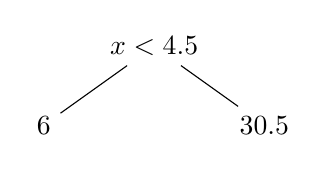
\begin{tikzpicture}
\node (t) at (0,1) {$x<4.5$};\node (l) at (-1.4,0) {$6$};\node (r) at (1.4,0) {$30.5$};\draw (t)--(l);\draw (t)--(r);
\end{tikzpicture}\end{center}
The dashed segments show the two leaf predictions; the curve and dots show the target function and training data.
\begin{center}
\begin{tikzpicture}[x=1.3cm,y=0.16cm]
\draw[->] (0,0)--(6.4,0) node[right] {$x$};\draw[->] (0,0)--(0,38) node[above] {$y$};
\node[below] at (1,0) {$ 1 $};
\node[below] at (2,0) {$ 2 $};
\node[below] at (3,0) {$ 3 $};
\node[below] at (4,0) {$ 4 $};
\node[below] at (5,0) {$ 5 $};
\node[below] at (6,0) {$ 6 $};
\draw[thin,domain=0:6,samples=65] plot (\x,{\x*\x+0});
\fill (0,0) circle (1.4pt);
\fill (1,1) circle (1.4pt);
\fill (2,4) circle (1.4pt);
\fill (3,9) circle (1.4pt);
\fill (4,16) circle (1.4pt);
\fill (5,25) circle (1.4pt);
\fill (6,36) circle (1.4pt);
\draw[thick,dashed] (0,6)--(4.5,6);\fill (0,6) circle (1.4pt);
\draw (4.5,6) circle (1.8pt);
\draw[thick,dashed] (4.5,30.5)--(6,30.5);\fill (4.5,30.5) circle (1.4pt);
\fill (6,30.5) circle (1.4pt);
\end{tikzpicture}
\end{center}
\par\endgroup

\subsection*{Exercise 2.6 - Split the left child}
Apply the same split-selection procedure within each child node. Allow one additional split in each child, producing a depth-2 tree.

The \textbf{\textit{training error}} is the prediction error on the observations used to build the tree. \textbf{\textit{Noise}} is random variation in the measured targets. \textbf{\textit{Overfitting}} occurs when a model adapts to sample-specific details or noise in a way that harms its predictions on new data.

Take the left child produced by the best split.

\begin{enumerate}
\item
List the observations contained in this child.

\item
Determine all candidate thresholds that can still split these observations into two non-empty groups.

\item
For every candidate, calculate the total child SSE.

\item
Select the best split.

\end{enumerate}
\begingroup\color{red}

\subsubsection*{Solution 2.6}
After the first split, the left child contains

\[
x=(0,1,2,3,4)
\qquad
y=(0,1,4,9,16)
\]

Its candidate thresholds are

\[
0.5,\ 1.5,\ 2.5,\ 3.5
\]

The corresponding total SSE values are approximately

\begingroup
\small
\setlength{\tabcolsep}{4pt}
\begin{longtable}{l|l}
threshold & total SSE \\
\hline
\endfirsthead
threshold & total SSE \\
\hline
\endhead
0.5 & 129.00 \\[1.5pt]
1.5 & 73.17 \\[1.5pt]
2.5 & 33.17 \\[1.5pt]
3.5 & 49.00 \\[1.5pt]
\end{longtable}
\endgroup
Thus the left child selects

\[
x<2.5
\]

\par\endgroup

\subsection*{Exercise 2.7 - Split the right child}
\begin{enumerate}
\item
List the observations in the right child and its candidate thresholds.

\item
If only two observations remain, how many candidate midpoints are possible?

\item
Calculate the total child SSE and determine the best split.

\end{enumerate}
\begingroup\color{red}

\subsubsection*{Solution 2.7}
The right child contains only

\[
x=(5,6)
\qquad
y=(25,36)
\]

There is only one candidate threshold:

\[
x<5.5.
\]

After that split each of these two observations occupies its own leaf,
so the SSE of this branch becomes zero.

\par\endgroup

\subsection*{Exercise 2.8 - Draw the depth-2 tree}
\begin{enumerate}
\item
Draw the complete depth-2 tree. Label every internal node with its split condition and every leaf with its constant prediction.

\item
Draw the corresponding step function $\hat f(x)$ in the same coordinate system as $f(x)=x^2$.

\end{enumerate}
\begingroup\color{red}

\subsubsection*{Solution 2.8}
The depth-2 tree is therefore

\begin{verbatim}
                    x < 4.5
                  /         \
             x < 2.5       x < 5.5
             /     \        /      \
          1.67     12.5    25       36
\end{verbatim}
The leaf predictions come from

\[
\frac{0+1+4}{3}\approx1.67,
\]

\[
\frac{9+16}{2}=12.5,
\]

and the single leaves $25$ and $36$.

The total training SSE is now approximately

\[
33.17,
\]

which is far below the depth-1 value

\[
234.5.
\]

In the sketch, the depth-2 prediction is

\[
\hat f(x)=\begin{cases}
5/3,&x<2.5,\\
12.5,&2.5\leq x<4.5,\\
25,&4.5\leq x<5.5,\\
36,&x\geq5.5.
\end{cases}
\]

Draw these horizontal segments over $0\leq x\leq6$, using the right-hand
region's value at each threshold. The exact total SSE is $199/6$.


The dashed segments give the depth-2 prediction. Filled left endpoints and open right endpoints indicate the split convention.
\begin{center}
\begin{tikzpicture}[x=1.3cm,y=0.16cm]
\draw[->] (0,0)--(6.4,0) node[right] {$x$};\draw[->] (0,0)--(0,38) node[above] {$y$};
\node[below] at (1,0) {$ 1 $};
\node[below] at (2,0) {$ 2 $};
\node[below] at (3,0) {$ 3 $};
\node[below] at (4,0) {$ 4 $};
\node[below] at (5,0) {$ 5 $};
\node[below] at (6,0) {$ 6 $};
\draw[thin,domain=0:6,samples=65] plot (\x,{\x*\x+0});
\fill (0,0) circle (1.4pt);
\fill (1,1) circle (1.4pt);
\fill (2,4) circle (1.4pt);
\fill (3,9) circle (1.4pt);
\fill (4,16) circle (1.4pt);
\fill (5,25) circle (1.4pt);
\fill (6,36) circle (1.4pt);
\draw[thick,dashed] (0,1.6666666666666667)--(2.5,1.6666666666666667);\fill (0,1.6666666666666667) circle (1.4pt);
\draw (2.5,1.6666666666666667) circle (1.8pt);
\draw[thick,dashed] (2.5,12.5)--(4.5,12.5);\fill (2.5,12.5) circle (1.4pt);
\draw (4.5,12.5) circle (1.8pt);
\draw[thick,dashed] (4.5,25)--(5.5,25);\fill (4.5,25) circle (1.4pt);
\draw (5.5,25) circle (1.8pt);
\draw[thick,dashed] (5.5,36)--(6,36);\fill (5.5,36) circle (1.4pt);
\fill (6,36) circle (1.4pt);
\end{tikzpicture}
\end{center}
\par\endgroup

\subsection*{Exercise 2.9 - Compare the approximations}
Use the errors already calculated to complete the table.

\begingroup
\small
\setlength{\tabcolsep}{4pt}
\begin{longtable}{l|l}
Model & Training SSE \\
\hline
\endfirsthead
Model & Training SSE \\
\hline
\endhead
One root leaf & $\phantom{0}$ \\[3pt]
Depth-1 tree & $\phantom{0}$ \\[3pt]
Depth-2 tree & $\phantom{0}$ \\[3pt]
\end{longtable}
\endgroup
Which of these three models has the smallest training error?

\begingroup\color{red}

\subsubsection*{Solution 2.9}
\begingroup
\small
\setlength{\tabcolsep}{4pt}
\begin{longtable}{l|l}
Model & Training SSE \\
\hline
\endfirsthead
Model & Training SSE \\
\hline
\endhead
One root leaf & $1092$ \\[1.5pt]
Depth-1 tree & $234.5$ \\[1.5pt]
Depth-2 tree & $199/6\approx33.17$ \\[1.5pt]
\end{longtable}
\endgroup
The depth-2 tree has the smallest training error.

\par\endgroup

\clearpage
\section*{Part III - More than one input feature}
A regression tree can choose not only where to split, but also which feature to split.

Consider the two-dimensional function

\[
f(x_1,x_2)=x_1^2+4x_2.
\]

We sample

\[
x_1\in\{0,1,2,3\},
\qquad
x_2\in\{0,1\}.
\]

The \textbf{\textit{feature space}} consists of all possible combinations of input values. An \textbf{\textit{axis-aligned split}} tests one feature at a time. In the $(x_1,x_2)$ plane, draw $x_1$ horizontally and $x_2$ vertically; such splits have boundaries parallel to a coordinate axis. In two dimensions, the resulting regions are rectangles, possibly unbounded.

\subsection*{Exercise 3.1 - Understand the function before building a tree}
First fix $x_2=0$.

Then

\[
f(x_1,0)=x_1^2.
\]

Now fix $x_2=1$.

Then

\[
f(x_1,1)=x_1^2+4.
\]

\begin{enumerate}
\item
Evaluate both functions at $x_1=0,1,2,3$.

\item
Complete the table.

\begingroup
\small
\setlength{\tabcolsep}{4pt}
\begin{longtable}{l|l|l}
$x_1$ & $x_2$ & $y=f(x_1,x_2)$ \\
\hline
\endfirsthead
$x_1$ & $x_2$ & $y=f(x_1,x_2)$ \\
\hline
\endhead
0 & 0 &  \\[3pt]
1 & 0 &  \\[3pt]
2 & 0 &  \\[3pt]
3 & 0 &  \\[3pt]
0 & 1 &  \\[3pt]
1 & 1 &  \\[3pt]
2 & 1 &  \\[3pt]
3 & 1 &  \\[3pt]
\end{longtable}
\endgroup
\item
In separate coordinate systems, plot $f(x_1,0)$ and $f(x_1,1)$ as functions of $x_1$.

\end{enumerate}
\begingroup\color{red}

\subsubsection*{Solution 3.1}
For

\[
f(x_1,x_2)=x_1^2+4x_2,
\]

the data are

\begingroup
\small
\setlength{\tabcolsep}{4pt}
\begin{longtable}{l|l|l}
$x_1$ & $x_2$ & $y$ \\
\hline
\endfirsthead
$x_1$ & $x_2$ & $y$ \\
\hline
\endhead
0 & 0 & 0 \\[1.5pt]
1 & 0 & 1 \\[1.5pt]
2 & 0 & 4 \\[1.5pt]
3 & 0 & 9 \\[1.5pt]
0 & 1 & 4 \\[1.5pt]
1 & 1 & 5 \\[1.5pt]
2 & 1 & 8 \\[1.5pt]
3 & 1 & 13 \\[1.5pt]
\end{longtable}
\endgroup
For $x_2=0$,

\[
f(x_1,0)=x_1^2,
\]

while for $x_2=1$,

\[
f(x_1,1)=x_1^2+4.
\]

Thus the second curve is shifted upward by $4$.


For $x_2=0$:
\begin{center}
\begin{tikzpicture}[x=1.3cm,y=0.38cm]
\draw[->] (0,0)--(3.4,0) node[right] {$x$};\draw[->] (0,0)--(0,11) node[above] {$y$};
\node[below] at (1,0) {$ 1 $};
\node[below] at (2,0) {$ 2 $};
\node[below] at (3,0) {$ 3 $};
\draw[thin,domain=0:3,samples=65] plot (\x,{\x*\x+0});
\fill (0,0) circle (1.4pt);
\fill (1,1) circle (1.4pt);
\fill (2,4) circle (1.4pt);
\fill (3,9) circle (1.4pt);
\end{tikzpicture}
\end{center}
For $x_2=1$:
\begin{center}
\begin{tikzpicture}[x=1.3cm,y=0.38cm]
\draw[->] (0,0)--(3.4,0) node[right] {$x$};\draw[->] (0,0)--(0,15) node[above] {$y$};
\node[below] at (1,0) {$ 1 $};
\node[below] at (2,0) {$ 2 $};
\node[below] at (3,0) {$ 3 $};
\draw[thin,domain=0:3,samples=65] plot (\x,{\x*\x+4});
\fill (0,4) circle (1.4pt);
\fill (1,5) circle (1.4pt);
\fill (2,8) circle (1.4pt);
\fill (3,13) circle (1.4pt);
\end{tikzpicture}
\end{center}
\par\endgroup

\subsection*{Exercise 3.2 - Which feature is chosen first?}
The tree may now test conditions involving either feature. For $x_1$ and $x_2$, these are 4 thresholds in total, 3 for conditions involving $x_1$ and one for $x_2$, thus, at the root node, the algorithm must compare four candidate splits.

Complete the following table by repeating the same steps as in Exercises 2.4-2.5:

\begin{enumerate}
\item
assign observations to the left and right child,

\item
calculate the mean target in each child,

\item
calculate the SSE in each child,

\item
add the two errors.

\begingroup
\small
\setlength{\tabcolsep}{4pt}
\begin{longtable}{l|l|l|l|l}
feature & threshold & mean left & mean right & total SSE \\
\hline
\endfirsthead
feature & threshold & mean left & mean right & total SSE \\
\hline
\endhead
$x_1$ & 0.5 &  &  &  \\[3pt]
$x_1$ & 1.5 &  &  &  \\[3pt]
$x_1$ & 2.5 &  &  &  \\[3pt]
$x_2$ & 0.5 &  &  &  \\[3pt]
\end{longtable}
\endgroup
Which feature and threshold are selected?

\end{enumerate}
\begingroup\color{red}

\subsubsection*{Solution 3.2}
The root candidate thresholds are

\[
x_1<0.5\qquad
x_1<1.5\qquad
x_1<2.5
\]

and

\[
x_2<0.5.
\]

The split comparison is

\begingroup
\small
\setlength{\tabcolsep}{4pt}
\begin{longtable}{l|l|l|l|l}
feature & threshold & mean left & mean right & total SSE \\
\hline
\endfirsthead
feature & threshold & mean left & mean right & total SSE \\
\hline
\endhead
$x_1$ & 0.5 & 2.00 & 6.67 & 97.33 \\[1.5pt]
$x_1$ & 1.5 & 2.50 & 8.50 & 58.00 \\[1.5pt]
$x_1$ & 2.5 & 3.67 & 11.00 & 49.33 \\[1.5pt]
$x_2$ & 0.5 & 3.50 & 7.50 & 98.00 \\[1.5pt]
\end{longtable}
\endgroup
Therefore the root selects

\[
x_1<2.5
\]

The depth-1 tree predicts the same value for $x_2=0$ and $x_2=1$
whenever the two observations fall into the same $x_1$ region, because
the root split has not used $x_2$ yet.

\par\endgroup

\subsection*{Exercise 3.3 - Grow one more level}
Now allow each child node to split once more.

For each child:

\begin{enumerate}
\item
determine which observations are present,

\item
determine which candidate splits are still possible,

\item
calculate their total SSE,

\item
choose the best split.

Draw the resulting depth-2 tree.

Then again sketch the prediction as a function of $x_1$

\begin{itemize}
\item
for $x_2=0$,

\item
for $x_2=1$.

\end{itemize}
\end{enumerate}
\begingroup\color{red}

\subsubsection*{Solution 3.3}
The left child contains $(x_1,x_2)$ with $x_1\in\{0,1,2\}$ and
$x_2\in\{0,1\}$, with targets $0,1,4,4,5,8$. Its candidate comparison
is:

\begingroup
\small
\setlength{\tabcolsep}{4pt}
\begin{longtable}{l|l|l|l|l}
Feature & Threshold & Mean left & Mean right & Total SSE \\
\hline
\endfirsthead
Feature & Threshold & Mean left & Mean right & Total SSE \\
\hline
\endhead
$x_1$ & 0.5 & 2.00 & 4.50 & 33.00 \\[1.5pt]
$x_1$ & 1.5 & 2.50 & 6.00 & 25.00 \\[1.5pt]
$x_2$ & 0.5 & 1.67 & 5.67 & 17.33 \\[1.5pt]
\end{longtable}
\endgroup
The best split is $x_2<0.5$. Its leaves predict $5/3$ and $17/3$, and
their total SSE is $52/3$.

The right child contains $(3,0,9)$ and $(3,1,13)$. The feature $x_1$ is
constant here, so it cannot split the node into two non-empty children:

\begingroup
\small
\setlength{\tabcolsep}{4pt}
\begin{longtable}{l|l|l|l|l}
Feature & Threshold & Mean left & Mean right & Total SSE \\
\hline
\endfirsthead
Feature & Threshold & Mean left & Mean right & Total SSE \\
\hline
\endhead
$x_2$ & 0.5 & 9.00 & 13.00 & 0.00 \\[1.5pt]
\end{longtable}
\endgroup
The only candidate is $x_2<0.5$; it gives leaf predictions $9$ and $13$
and zero SSE.

\begin{verbatim}
                      x1 < 2.5
                    /          \
               x2 < 0.5      x2 < 0.5
               /      \      /      \
             5/3     17/3    9       13
\end{verbatim}
Every left branch means the condition is true; every right branch means
it is false. For the requested sketches,

\[
\hat f(x_1,0)=\begin{cases}5/3,&x_1<2.5,\\9,&x_1\geq2.5,\end{cases}
\qquad
\hat f(x_1,1)=\begin{cases}17/3,&x_1<2.5,\\13,&x_1\geq2.5.\end{cases}
\]

The two step functions now differ by $4$, reflecting the effect of the
second feature. Draw the curves $x_1^2$ and $x_1^2+4$ behind them for
comparison.

The total training SSE falls from $148/3\approx49.33$ at depth 1 to
$52/3\approx17.33$ at depth 2. Each individual split uses one feature,
while different nodes can use different features. Together these splits
define rectangular regions, with a constant prediction in each region.


For $x_2=0$, the dashed segments are $5/3$ and $9$:
\begin{center}
\begin{tikzpicture}[x=1.3cm,y=0.38cm]
\draw[->] (0,0)--(3.4,0) node[right] {$x$};\draw[->] (0,0)--(0,11) node[above] {$y$};
\node[below] at (1,0) {$ 1 $};
\node[below] at (2,0) {$ 2 $};
\node[below] at (3,0) {$ 3 $};
\draw[thin,domain=0:3,samples=65] plot (\x,{\x*\x+0});
\fill (0,0) circle (1.4pt);
\fill (1,1) circle (1.4pt);
\fill (2,4) circle (1.4pt);
\fill (3,9) circle (1.4pt);
\draw[thick,dashed] (0,1.6666666666666667)--(2.5,1.6666666666666667);\fill (0,1.6666666666666667) circle (1.4pt);
\draw (2.5,1.6666666666666667) circle (1.8pt);
\draw[thick,dashed] (2.5,9)--(3,9);\fill (2.5,9) circle (1.4pt);
\fill (3,9) circle (1.4pt);
\end{tikzpicture}
\end{center}
For $x_2=1$, they are $17/3$ and $13$:
\begin{center}
\begin{tikzpicture}[x=1.3cm,y=0.38cm]
\draw[->] (0,0)--(3.4,0) node[right] {$x$};\draw[->] (0,0)--(0,15) node[above] {$y$};
\node[below] at (1,0) {$ 1 $};
\node[below] at (2,0) {$ 2 $};
\node[below] at (3,0) {$ 3 $};
\draw[thin,domain=0:3,samples=65] plot (\x,{\x*\x+4});
\fill (0,4) circle (1.4pt);
\fill (1,5) circle (1.4pt);
\fill (2,8) circle (1.4pt);
\fill (3,13) circle (1.4pt);
\draw[thick,dashed] (0,5.666666666666667)--(2.5,5.666666666666667);\fill (0,5.666666666666667) circle (1.4pt);
\draw (2.5,5.666666666666667) circle (1.8pt);
\draw[thick,dashed] (2.5,13)--(3,13);\fill (2.5,13) circle (1.4pt);
\fill (3,13) circle (1.4pt);
\end{tikzpicture}
\end{center}
\par\endgroup

\clearpage
\section*{Part IV - A forest by hand}
You will first train a regression tree using absolute error. You will then train three trees on bootstrap samples, average their predictions to form a forest, and compare the predictions with those of the single tree.

\subsection*{Exercise 4.1 - Training data}
Consider

\[
f(x)=\sin(x)+\frac{x}{\pi},\qquad 0\leq x\leq2\pi.
\]

Each input position occurs exactly once in the training dataset.

\begingroup
\small
\setlength{\tabcolsep}{4pt}
\begin{longtable}{l|l}
$x$ & $f(x)$ \\
\hline
\endfirsthead
$x$ & $f(x)$ \\
\hline
\endhead
$0$ & $\phantom{0}$ \\[3pt]
$\pi/2$ & $\phantom{0}$ \\[3pt]
$\pi$ & $\phantom{0}$ \\[3pt]
$3\pi/2$ & $\phantom{0}$ \\[3pt]
$2\pi$ & $\phantom{0}$ \\[3pt]
\end{longtable}
\endgroup
\begin{enumerate}
\item
Complete the table.

\item
Plot the five training points and sketch the function.

\end{enumerate}
\begingroup\color{red}

\subsubsection*{Solution 4.1}
\begingroup
\small
\setlength{\tabcolsep}{4pt}
\begin{longtable}{l|l}
$x$ & $f(x)$ \\
\hline
\endfirsthead
$x$ & $f(x)$ \\
\hline
\endhead
$0$ & $0$ \\[1.5pt]
$\pi/2$ & $\frac{3}{2}$ \\[1.5pt]
$\pi$ & $1$ \\[1.5pt]
$3\pi/2$ & $\frac{1}{2}$ \\[1.5pt]
$2\pi$ & $2$ \\[1.5pt]
\end{longtable}
\endgroup
There are five observations with no repetitions. For the sketch, add the
sine curve to the line $y=x/\pi$.


The solid curve is $\sin(x)+x/\pi$; dots mark the five distinct training inputs.
\begin{center}
\begin{tikzpicture}[x=3.5cm,y=1.8cm]
\draw[->] (0,0)--(2.2,0) node[right] {$x$};\draw[->] (0,0)--(0,2.4) node[above] {$y$};
\foreach \x/\lab in {0/0,0.5/{\pi/2},1/\pi,1.5/{3\pi/2},2/{2\pi}} {\node[below] at (\x,0) {$\lab$};}
\foreach \y in {0.5,1,1.5,2} {\node[left] at (0,\y) {$\y$};}
\draw[thin,domain=0:2,samples=121] plot (\x,{sin(180*\x)+\x});
\foreach \x/\y in {0/0,0.5/1.5,1/1,1.5/0.5,2/2} {\fill (\x,\y) circle (1.4pt);}
\end{tikzpicture}
\end{center}
\par\endgroup

\subsection*{Exercise 4.2 - Train a tree using absolute error}
The \textbf{\textit{median}} is the middle value of a sorted list. For an odd number of values, take the single middle value. For an even number, use the arithmetic mean of the two middle values.

For example, the median of $1,3,8$ is $3$, and the median of $1,3,5,8$ is $(3+5)/2=4$.

A leaf prediction $c$ has mean absolute error

\[
\mathrm{MAE}(c)=\frac1N\sum_{i=1}^{N}|y_i-c|.
\]

A median minimizes this error. Determine the leaf median by sorting the \textbf{\textit{target values}}.

For each threshold, send $x<t$ to the left child and $x\geq t$ to the right child. The child sets are given below. Dashes mark unused cells. Fill in the function values and enter each child's median and MAE in its $f(x_i)$ row.

\paragraph*{Threshold $t=\pi/4$}
\begingroup
\small
\setlength{\tabcolsep}{4pt}
\begin{longtable}{l|l|l|l|l|l|l|l}
Child &  & 1 & 2 & 3 & 4 & Median & MAE \\
\hline
\endfirsthead
Child &  & 1 & 2 & 3 & 4 & Median & MAE \\
\hline
\endhead
L & $x_i$ & $0$ & - & - & - & - & - \\[3pt]
 & $f(x_i)$ & $\phantom{0}$ & - & - & - & $\phantom{0}$ & $\phantom{0}$ \\[3pt]
R & $x_i$ & $\pi/2$ & $\pi$ & $3\pi/2$ & $2\pi$ & - & - \\[3pt]
 & $f(x_i)$ & $\phantom{0}$ & $\phantom{0}$ & $\phantom{0}$ & $\phantom{0}$ & $\phantom{0}$ & $\phantom{0}$ \\[3pt]
\end{longtable}
\endgroup
\paragraph*{Threshold $t=3\pi/4$}
\begingroup
\small
\setlength{\tabcolsep}{4pt}
\begin{longtable}{l|l|l|l|l|l|l}
Child &  & 1 & 2 & 3 & Median & MAE \\
\hline
\endfirsthead
Child &  & 1 & 2 & 3 & Median & MAE \\
\hline
\endhead
L & $x_i$ & $0$ & $\pi/2$ & - & - & - \\[3pt]
 & $f(x_i)$ & $\phantom{0}$ & $\phantom{0}$ & - & $\phantom{0}$ & $\phantom{0}$ \\[3pt]
R & $x_i$ & $\pi$ & $3\pi/2$ & $2\pi$ & - & - \\[3pt]
 & $f(x_i)$ & $\phantom{0}$ & $\phantom{0}$ & $\phantom{0}$ & $\phantom{0}$ & $\phantom{0}$ \\[3pt]
\end{longtable}
\endgroup
\paragraph*{Threshold $t=5\pi/4$}
\begingroup
\small
\setlength{\tabcolsep}{4pt}
\begin{longtable}{l|l|l|l|l|l|l}
Child &  & 1 & 2 & 3 & Median & MAE \\
\hline
\endfirsthead
Child &  & 1 & 2 & 3 & Median & MAE \\
\hline
\endhead
L & $x_i$ & $0$ & $\pi/2$ & $\pi$ & - & - \\[3pt]
 & $f(x_i)$ & $\phantom{0}$ & $\phantom{0}$ & $\phantom{0}$ & $\phantom{0}$ & $\phantom{0}$ \\[3pt]
R & $x_i$ & $3\pi/2$ & $2\pi$ & - & - & - \\[3pt]
 & $f(x_i)$ & $\phantom{0}$ & $\phantom{0}$ & - & $\phantom{0}$ & $\phantom{0}$ \\[3pt]
\end{longtable}
\endgroup
\paragraph*{Threshold $t=7\pi/4$}
\begingroup
\small
\setlength{\tabcolsep}{4pt}
\begin{longtable}{l|l|l|l|l|l|l|l}
Child &  & 1 & 2 & 3 & 4 & Median & MAE \\
\hline
\endfirsthead
Child &  & 1 & 2 & 3 & 4 & Median & MAE \\
\hline
\endhead
L & $x_i$ & $0$ & $\pi/2$ & $\pi$ & $3\pi/2$ & - & - \\[3pt]
 & $f(x_i)$ & $\phantom{0}$ & $\phantom{0}$ & $\phantom{0}$ & $\phantom{0}$ & $\phantom{0}$ & $\phantom{0}$ \\[3pt]
R & $x_i$ & $2\pi$ & - & - & - & - & - \\[3pt]
 & $f(x_i)$ & $\phantom{0}$ & - & - & - & $\phantom{0}$ & $\phantom{0}$ \\[3pt]
\end{longtable}
\endgroup
\subsubsection*{Compare the thresholds}
\begin{enumerate}
\item
Complete the four tables above.

\item
Calculate the total absolute error for each threshold:

\[
S=N_L\mathrm{MAE}_L+N_R\mathrm{MAE}_R,
\]

where $N_L$ and $N_R$ are the numbers of observations in the children.

\item
Enter the results below.

\end{enumerate}
\begingroup
\small
\setlength{\tabcolsep}{4pt}
\begin{longtable}{l|l}
Threshold & Sum $S$ \\
\hline
\endfirsthead
Threshold & Sum $S$ \\
\hline
\endhead
$\pi/4$ & $\phantom{0}$ \\[3pt]
$3\pi/4$ & $\phantom{0}$ \\[3pt]
$5\pi/4$ & $\phantom{0}$ \\[3pt]
$7\pi/4$ & $\phantom{0}$ \\[3pt]
\end{longtable}
\endgroup
\begin{enumerate}
\setcounter{enumi}{3}
\item
Select the threshold with the smallest $S$. If thresholds give the same error, choose the smaller threshold.

\item
Draw the depth-1 tree and label its leaves with their median predictions.

\item
Calculate the tree's training MAE as $S/5$.

\item
Calculate the median and MAE of the unsplit dataset. Compare the errors before and after splitting.

\end{enumerate}
\begingroup\color{red}

\subsubsection*{Solution 4.2}
The completed tables give the target values in increasing input order.
Sort them within each child to determine its median.

\paragraph*{Threshold $t=\pi/4$}
\begingroup
\small
\setlength{\tabcolsep}{4pt}
\begin{longtable}{l|l|l|l|l|l|l|l}
Child &  & 1 & 2 & 3 & 4 & Median & MAE \\
\hline
\endfirsthead
Child &  & 1 & 2 & 3 & 4 & Median & MAE \\
\hline
\endhead
L & $x_i$ & $0$ & - & - & - & - & - \\[3pt]
 & $f(x_i)$ & $0$ & - & - & - & $0$ & $0$ \\[3pt]
R & $x_i$ & $\pi/2$ & $\pi$ & $3\pi/2$ & $2\pi$ & - & - \\[3pt]
 & $f(x_i)$ & $\frac{3}{2}$ & $1$ & $\frac{1}{2}$ & $2$ & $\frac{5}{4}$ & $\frac{1}{2}$ \\[3pt]
\end{longtable}
\endgroup
\paragraph*{Threshold $t=3\pi/4$}
\begingroup
\small
\setlength{\tabcolsep}{4pt}
\begin{longtable}{l|l|l|l|l|l|l}
Child &  & 1 & 2 & 3 & Median & MAE \\
\hline
\endfirsthead
Child &  & 1 & 2 & 3 & Median & MAE \\
\hline
\endhead
L & $x_i$ & $0$ & $\pi/2$ & - & - & - \\[3pt]
 & $f(x_i)$ & $0$ & $\frac{3}{2}$ & - & $\frac{3}{4}$ & $\frac{3}{4}$ \\[3pt]
R & $x_i$ & $\pi$ & $3\pi/2$ & $2\pi$ & - & - \\[3pt]
 & $f(x_i)$ & $1$ & $\frac{1}{2}$ & $2$ & $1$ & $\frac{1}{2}$ \\[3pt]
\end{longtable}
\endgroup
\paragraph*{Threshold $t=5\pi/4$}
\begingroup
\small
\setlength{\tabcolsep}{4pt}
\begin{longtable}{l|l|l|l|l|l|l}
Child &  & 1 & 2 & 3 & Median & MAE \\
\hline
\endfirsthead
Child &  & 1 & 2 & 3 & Median & MAE \\
\hline
\endhead
L & $x_i$ & $0$ & $\pi/2$ & $\pi$ & - & - \\[3pt]
 & $f(x_i)$ & $0$ & $\frac{3}{2}$ & $1$ & $1$ & $\frac{1}{2}$ \\[3pt]
R & $x_i$ & $3\pi/2$ & $2\pi$ & - & - & - \\[3pt]
 & $f(x_i)$ & $\frac{1}{2}$ & $2$ & - & $\frac{5}{4}$ & $\frac{3}{4}$ \\[3pt]
\end{longtable}
\endgroup
\paragraph*{Threshold $t=7\pi/4$}
\begingroup
\small
\setlength{\tabcolsep}{4pt}
\begin{longtable}{l|l|l|l|l|l|l|l}
Child &  & 1 & 2 & 3 & 4 & Median & MAE \\
\hline
\endfirsthead
Child &  & 1 & 2 & 3 & 4 & Median & MAE \\
\hline
\endhead
L & $x_i$ & $0$ & $\pi/2$ & $\pi$ & $3\pi/2$ & - & - \\[3pt]
 & $f(x_i)$ & $0$ & $\frac{3}{2}$ & $1$ & $\frac{1}{2}$ & $\frac{3}{4}$ & $\frac{1}{2}$ \\[3pt]
R & $x_i$ & $2\pi$ & - & - & - & - & - \\[3pt]
 & $f(x_i)$ & $2$ & - & - & - & $2$ & $0$ \\[3pt]
\end{longtable}
\endgroup
\begingroup
\small
\setlength{\tabcolsep}{4pt}
\begin{longtable}{l|l}
Threshold & Sum $S$ \\
\hline
\endfirsthead
Threshold & Sum $S$ \\
\hline
\endhead
$\pi/4$ & $2$ \\[1.5pt]
$3\pi/4$ & $3$ \\[1.5pt]
$5\pi/4$ & $3$ \\[1.5pt]
$7\pi/4$ & $2$ \\[1.5pt]
\end{longtable}
\endgroup
For $t=\pi/4$, the right targets sort to $1/2,1,3/2,2$. Their median is
$5/4$, and their MAE is $(3/4+1/4+1/4+3/4)/4=1/2$.

The thresholds $\pi/4$ and $7\pi/4$ tie. The prescribed rule selects
$\pi/4$:

\begin{center}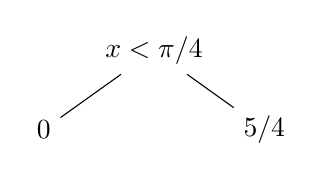
\begin{tikzpicture}
\node (t) at (0,1) {$x<\pi/4$};\node (l) at (-1.4,0) {$0$};\node (r) at (1.4,0) {$5/4$};\draw (t)--(l);\draw (t)--(r);
\end{tikzpicture}\end{center}

\[
\hat f_{\mathrm{single}}(x)=\begin{cases}0,&x<\pi/4,\\5/4,&x\geq\pi/4.\end{cases}
\]

Its training MAE is $2/5$. The unsplit targets sort to $0,1/2,1,3/2,2$,
with median $1$ and MAE $(1+1/2+0+1/2+1)/5=3/5$.

\par\endgroup

\subsection*{Exercise 4.3 - Train three trees}
A \textbf{\textit{bootstrap sample}} is obtained by drawing observations with replacement from the training dataset. After each draw, all original observations remain available for the next draw. An observation can therefore occur several times or be absent from a sample.

Use five draws per tree. Three possible samples are specified below; each column sums to five.

\begingroup
\small
\setlength{\tabcolsep}{4pt}
\begin{longtable}{l|l|l|l}
$x$ & Sample A & Sample B & Sample C \\
\hline
\endfirsthead
$x$ & Sample A & Sample B & Sample C \\
\hline
\endhead
$0$ & 2 & 1 & 2 \\[1.5pt]
$\pi/2$ & 1 & 0 & 0 \\[1.5pt]
$\pi$ & 1 & 1 & 2 \\[1.5pt]
$3\pi/2$ & 0 & 1 & 0 \\[1.5pt]
$2\pi$ & 1 & 2 & 1 \\[1.5pt]
\end{longtable}
\endgroup
Train one depth-1 tree per sample using the prepared tables below.

\begin{enumerate}
\item
Fill in the function values and calculate the median and MAE for each child. Count each repeated observation separately when sorting targets and calculating errors.

\item
Complete the summary table for each sample using $S=N_L\mathrm{MAE}_L+N_R\mathrm{MAE}_R$.

\item
Select the best split using the rule from Exercise 4.2.

\item
Draw each tree and write its prediction as a piecewise-constant function.

\end{enumerate}
The candidate thresholds are the midpoints between neighboring distinct input values present in each sample.

\subsubsection*{Sample A}
\paragraph*{Threshold $t=\pi/4$}
\begingroup
\small
\setlength{\tabcolsep}{4pt}
\begin{longtable}{l|l|l|l|l|l|l}
Child &  & 1 & 2 & 3 & Median & MAE \\
\hline
\endfirsthead
Child &  & 1 & 2 & 3 & Median & MAE \\
\hline
\endhead
L & $x_i$ & $0$ & $0$ & - & - & - \\[3pt]
 & $f(x_i)$ & $\phantom{0}$ & $\phantom{0}$ & - & $\phantom{0}$ & $\phantom{0}$ \\[3pt]
R & $x_i$ & $\pi/2$ & $\pi$ & $2\pi$ & - & - \\[3pt]
 & $f(x_i)$ & $\phantom{0}$ & $\phantom{0}$ & $\phantom{0}$ & $\phantom{0}$ & $\phantom{0}$ \\[3pt]
\end{longtable}
\endgroup
\paragraph*{Threshold $t=3\pi/4$}
\begingroup
\small
\setlength{\tabcolsep}{4pt}
\begin{longtable}{l|l|l|l|l|l|l}
Child &  & 1 & 2 & 3 & Median & MAE \\
\hline
\endfirsthead
Child &  & 1 & 2 & 3 & Median & MAE \\
\hline
\endhead
L & $x_i$ & $0$ & $0$ & $\pi/2$ & - & - \\[3pt]
 & $f(x_i)$ & $\phantom{0}$ & $\phantom{0}$ & $\phantom{0}$ & $\phantom{0}$ & $\phantom{0}$ \\[3pt]
R & $x_i$ & $\pi$ & $2\pi$ & - & - & - \\[3pt]
 & $f(x_i)$ & $\phantom{0}$ & $\phantom{0}$ & - & $\phantom{0}$ & $\phantom{0}$ \\[3pt]
\end{longtable}
\endgroup
\paragraph*{Threshold $t=3\pi/2$}
\begingroup
\small
\setlength{\tabcolsep}{4pt}
\begin{longtable}{l|l|l|l|l|l|l|l}
Child &  & 1 & 2 & 3 & 4 & Median & MAE \\
\hline
\endfirsthead
Child &  & 1 & 2 & 3 & 4 & Median & MAE \\
\hline
\endhead
L & $x_i$ & $0$ & $0$ & $\pi/2$ & $\pi$ & - & - \\[3pt]
 & $f(x_i)$ & $\phantom{0}$ & $\phantom{0}$ & $\phantom{0}$ & $\phantom{0}$ & $\phantom{0}$ & $\phantom{0}$ \\[3pt]
R & $x_i$ & $2\pi$ & - & - & - & - & - \\[3pt]
 & $f(x_i)$ & $\phantom{0}$ & - & - & - & $\phantom{0}$ & $\phantom{0}$ \\[3pt]
\end{longtable}
\endgroup
\begingroup
\small
\setlength{\tabcolsep}{4pt}
\begin{longtable}{l|l}
Threshold & Sum $S$ \\
\hline
\endfirsthead
Threshold & Sum $S$ \\
\hline
\endhead
$\pi/4$ & $\phantom{0}$ \\[3pt]
$3\pi/4$ & $\phantom{0}$ \\[3pt]
$3\pi/2$ & $\phantom{0}$ \\[3pt]
\end{longtable}
\endgroup
\subsubsection*{Sample B}
\paragraph*{Threshold $t=\pi/2$}
\begingroup
\small
\setlength{\tabcolsep}{4pt}
\begin{longtable}{l|l|l|l|l|l|l|l}
Child &  & 1 & 2 & 3 & 4 & Median & MAE \\
\hline
\endfirsthead
Child &  & 1 & 2 & 3 & 4 & Median & MAE \\
\hline
\endhead
L & $x_i$ & $0$ & - & - & - & - & - \\[3pt]
 & $f(x_i)$ & $\phantom{0}$ & - & - & - & $\phantom{0}$ & $\phantom{0}$ \\[3pt]
R & $x_i$ & $\pi$ & $3\pi/2$ & $2\pi$ & $2\pi$ & - & - \\[3pt]
 & $f(x_i)$ & $\phantom{0}$ & $\phantom{0}$ & $\phantom{0}$ & $\phantom{0}$ & $\phantom{0}$ & $\phantom{0}$ \\[3pt]
\end{longtable}
\endgroup
\paragraph*{Threshold $t=5\pi/4$}
\begingroup
\small
\setlength{\tabcolsep}{4pt}
\begin{longtable}{l|l|l|l|l|l|l}
Child &  & 1 & 2 & 3 & Median & MAE \\
\hline
\endfirsthead
Child &  & 1 & 2 & 3 & Median & MAE \\
\hline
\endhead
L & $x_i$ & $0$ & $\pi$ & - & - & - \\[3pt]
 & $f(x_i)$ & $\phantom{0}$ & $\phantom{0}$ & - & $\phantom{0}$ & $\phantom{0}$ \\[3pt]
R & $x_i$ & $3\pi/2$ & $2\pi$ & $2\pi$ & - & - \\[3pt]
 & $f(x_i)$ & $\phantom{0}$ & $\phantom{0}$ & $\phantom{0}$ & $\phantom{0}$ & $\phantom{0}$ \\[3pt]
\end{longtable}
\endgroup
\paragraph*{Threshold $t=7\pi/4$}
\begingroup
\small
\setlength{\tabcolsep}{4pt}
\begin{longtable}{l|l|l|l|l|l|l}
Child &  & 1 & 2 & 3 & Median & MAE \\
\hline
\endfirsthead
Child &  & 1 & 2 & 3 & Median & MAE \\
\hline
\endhead
L & $x_i$ & $0$ & $\pi$ & $3\pi/2$ & - & - \\[3pt]
 & $f(x_i)$ & $\phantom{0}$ & $\phantom{0}$ & $\phantom{0}$ & $\phantom{0}$ & $\phantom{0}$ \\[3pt]
R & $x_i$ & $2\pi$ & $2\pi$ & - & - & - \\[3pt]
 & $f(x_i)$ & $\phantom{0}$ & $\phantom{0}$ & - & $\phantom{0}$ & $\phantom{0}$ \\[3pt]
\end{longtable}
\endgroup
\begingroup
\small
\setlength{\tabcolsep}{4pt}
\begin{longtable}{l|l}
Threshold & Sum $S$ \\
\hline
\endfirsthead
Threshold & Sum $S$ \\
\hline
\endhead
$\pi/2$ & $\phantom{0}$ \\[3pt]
$5\pi/4$ & $\phantom{0}$ \\[3pt]
$7\pi/4$ & $\phantom{0}$ \\[3pt]
\end{longtable}
\endgroup
\subsubsection*{Sample C}
\paragraph*{Threshold $t=\pi/2$}
\begingroup
\small
\setlength{\tabcolsep}{4pt}
\begin{longtable}{l|l|l|l|l|l|l}
Child &  & 1 & 2 & 3 & Median & MAE \\
\hline
\endfirsthead
Child &  & 1 & 2 & 3 & Median & MAE \\
\hline
\endhead
L & $x_i$ & $0$ & $0$ & - & - & - \\[3pt]
 & $f(x_i)$ & $\phantom{0}$ & $\phantom{0}$ & - & $\phantom{0}$ & $\phantom{0}$ \\[3pt]
R & $x_i$ & $\pi$ & $\pi$ & $2\pi$ & - & - \\[3pt]
 & $f(x_i)$ & $\phantom{0}$ & $\phantom{0}$ & $\phantom{0}$ & $\phantom{0}$ & $\phantom{0}$ \\[3pt]
\end{longtable}
\endgroup
\paragraph*{Threshold $t=3\pi/2$}
\begingroup
\small
\setlength{\tabcolsep}{4pt}
\begin{longtable}{l|l|l|l|l|l|l|l}
Child &  & 1 & 2 & 3 & 4 & Median & MAE \\
\hline
\endfirsthead
Child &  & 1 & 2 & 3 & 4 & Median & MAE \\
\hline
\endhead
L & $x_i$ & $0$ & $0$ & $\pi$ & $\pi$ & - & - \\[3pt]
 & $f(x_i)$ & $\phantom{0}$ & $\phantom{0}$ & $\phantom{0}$ & $\phantom{0}$ & $\phantom{0}$ & $\phantom{0}$ \\[3pt]
R & $x_i$ & $2\pi$ & - & - & - & - & - \\[3pt]
 & $f(x_i)$ & $\phantom{0}$ & - & - & - & $\phantom{0}$ & $\phantom{0}$ \\[3pt]
\end{longtable}
\endgroup
\begingroup
\small
\setlength{\tabcolsep}{4pt}
\begin{longtable}{l|l}
Threshold & Sum $S$ \\
\hline
\endfirsthead
Threshold & Sum $S$ \\
\hline
\endhead
$\pi/2$ & $\phantom{0}$ \\[3pt]
$3\pi/2$ & $\phantom{0}$ \\[3pt]
\end{longtable}
\endgroup
\begingroup\color{red}

\subsubsection*{Solution 4.3}
\subsubsection*{Sample A}
\paragraph*{Threshold $t=\pi/4$}
\begingroup
\small
\setlength{\tabcolsep}{4pt}
\begin{longtable}{l|l|l|l|l|l|l}
Child &  & 1 & 2 & 3 & Median & MAE \\
\hline
\endfirsthead
Child &  & 1 & 2 & 3 & Median & MAE \\
\hline
\endhead
L & $x_i$ & $0$ & $0$ & - & - & - \\[3pt]
 & $f(x_i)$ & $0$ & $0$ & - & $0$ & $0$ \\[3pt]
R & $x_i$ & $\pi/2$ & $\pi$ & $2\pi$ & - & - \\[3pt]
 & $f(x_i)$ & $\frac{3}{2}$ & $1$ & $2$ & $\frac{3}{2}$ & $\frac{1}{3}$ \\[3pt]
\end{longtable}
\endgroup
\paragraph*{Threshold $t=3\pi/4$}
\begingroup
\small
\setlength{\tabcolsep}{4pt}
\begin{longtable}{l|l|l|l|l|l|l}
Child &  & 1 & 2 & 3 & Median & MAE \\
\hline
\endfirsthead
Child &  & 1 & 2 & 3 & Median & MAE \\
\hline
\endhead
L & $x_i$ & $0$ & $0$ & $\pi/2$ & - & - \\[3pt]
 & $f(x_i)$ & $0$ & $0$ & $\frac{3}{2}$ & $0$ & $\frac{1}{2}$ \\[3pt]
R & $x_i$ & $\pi$ & $2\pi$ & - & - & - \\[3pt]
 & $f(x_i)$ & $1$ & $2$ & - & $\frac{3}{2}$ & $\frac{1}{2}$ \\[3pt]
\end{longtable}
\endgroup
\paragraph*{Threshold $t=3\pi/2$}
\begingroup
\small
\setlength{\tabcolsep}{4pt}
\begin{longtable}{l|l|l|l|l|l|l|l}
Child &  & 1 & 2 & 3 & 4 & Median & MAE \\
\hline
\endfirsthead
Child &  & 1 & 2 & 3 & 4 & Median & MAE \\
\hline
\endhead
L & $x_i$ & $0$ & $0$ & $\pi/2$ & $\pi$ & - & - \\[3pt]
 & $f(x_i)$ & $0$ & $0$ & $\frac{3}{2}$ & $1$ & $\frac{1}{2}$ & $\frac{5}{8}$ \\[3pt]
R & $x_i$ & $2\pi$ & - & - & - & - & - \\[3pt]
 & $f(x_i)$ & $2$ & - & - & - & $2$ & $0$ \\[3pt]
\end{longtable}
\endgroup
\begingroup
\small
\setlength{\tabcolsep}{4pt}
\begin{longtable}{l|l}
Threshold & Sum $S$ \\
\hline
\endfirsthead
Threshold & Sum $S$ \\
\hline
\endhead
$\pi/4$ & $1$ \\[1.5pt]
$3\pi/4$ & $\frac{5}{2}$ \\[1.5pt]
$3\pi/2$ & $\frac{5}{2}$ \\[1.5pt]
\end{longtable}
\endgroup
The best split gives

\[
\hat f_A(x)=\begin{cases}0,&x<\pi/4,\\\frac{3}{2},&x\geq \pi/4.\end{cases}
\]

\subsubsection*{Sample B}
\paragraph*{Threshold $t=\pi/2$}
\begingroup
\small
\setlength{\tabcolsep}{4pt}
\begin{longtable}{l|l|l|l|l|l|l|l}
Child &  & 1 & 2 & 3 & 4 & Median & MAE \\
\hline
\endfirsthead
Child &  & 1 & 2 & 3 & 4 & Median & MAE \\
\hline
\endhead
L & $x_i$ & $0$ & - & - & - & - & - \\[3pt]
 & $f(x_i)$ & $0$ & - & - & - & $0$ & $0$ \\[3pt]
R & $x_i$ & $\pi$ & $3\pi/2$ & $2\pi$ & $2\pi$ & - & - \\[3pt]
 & $f(x_i)$ & $1$ & $\frac{1}{2}$ & $2$ & $2$ & $\frac{3}{2}$ & $\frac{5}{8}$ \\[3pt]
\end{longtable}
\endgroup
\paragraph*{Threshold $t=5\pi/4$}
\begingroup
\small
\setlength{\tabcolsep}{4pt}
\begin{longtable}{l|l|l|l|l|l|l}
Child &  & 1 & 2 & 3 & Median & MAE \\
\hline
\endfirsthead
Child &  & 1 & 2 & 3 & Median & MAE \\
\hline
\endhead
L & $x_i$ & $0$ & $\pi$ & - & - & - \\[3pt]
 & $f(x_i)$ & $0$ & $1$ & - & $\frac{1}{2}$ & $\frac{1}{2}$ \\[3pt]
R & $x_i$ & $3\pi/2$ & $2\pi$ & $2\pi$ & - & - \\[3pt]
 & $f(x_i)$ & $\frac{1}{2}$ & $2$ & $2$ & $2$ & $\frac{1}{2}$ \\[3pt]
\end{longtable}
\endgroup
\paragraph*{Threshold $t=7\pi/4$}
\begingroup
\small
\setlength{\tabcolsep}{4pt}
\begin{longtable}{l|l|l|l|l|l|l}
Child &  & 1 & 2 & 3 & Median & MAE \\
\hline
\endfirsthead
Child &  & 1 & 2 & 3 & Median & MAE \\
\hline
\endhead
L & $x_i$ & $0$ & $\pi$ & $3\pi/2$ & - & - \\[3pt]
 & $f(x_i)$ & $0$ & $1$ & $\frac{1}{2}$ & $\frac{1}{2}$ & $\frac{1}{3}$ \\[3pt]
R & $x_i$ & $2\pi$ & $2\pi$ & - & - & - \\[3pt]
 & $f(x_i)$ & $2$ & $2$ & - & $2$ & $0$ \\[3pt]
\end{longtable}
\endgroup
\begingroup
\small
\setlength{\tabcolsep}{4pt}
\begin{longtable}{l|l}
Threshold & Sum $S$ \\
\hline
\endfirsthead
Threshold & Sum $S$ \\
\hline
\endhead
$\pi/2$ & $\frac{5}{2}$ \\[1.5pt]
$5\pi/4$ & $\frac{5}{2}$ \\[1.5pt]
$7\pi/4$ & $1$ \\[1.5pt]
\end{longtable}
\endgroup
The best split gives

\[
\hat f_B(x)=\begin{cases}\frac{1}{2},&x<7\pi/4,\\2,&x\geq 7\pi/4.\end{cases}
\]

\subsubsection*{Sample C}
\paragraph*{Threshold $t=\pi/2$}
\begingroup
\small
\setlength{\tabcolsep}{4pt}
\begin{longtable}{l|l|l|l|l|l|l}
Child &  & 1 & 2 & 3 & Median & MAE \\
\hline
\endfirsthead
Child &  & 1 & 2 & 3 & Median & MAE \\
\hline
\endhead
L & $x_i$ & $0$ & $0$ & - & - & - \\[3pt]
 & $f(x_i)$ & $0$ & $0$ & - & $0$ & $0$ \\[3pt]
R & $x_i$ & $\pi$ & $\pi$ & $2\pi$ & - & - \\[3pt]
 & $f(x_i)$ & $1$ & $1$ & $2$ & $1$ & $\frac{1}{3}$ \\[3pt]
\end{longtable}
\endgroup
\paragraph*{Threshold $t=3\pi/2$}
\begingroup
\small
\setlength{\tabcolsep}{4pt}
\begin{longtable}{l|l|l|l|l|l|l|l}
Child &  & 1 & 2 & 3 & 4 & Median & MAE \\
\hline
\endfirsthead
Child &  & 1 & 2 & 3 & 4 & Median & MAE \\
\hline
\endhead
L & $x_i$ & $0$ & $0$ & $\pi$ & $\pi$ & - & - \\[3pt]
 & $f(x_i)$ & $0$ & $0$ & $1$ & $1$ & $\frac{1}{2}$ & $\frac{1}{2}$ \\[3pt]
R & $x_i$ & $2\pi$ & - & - & - & - & - \\[3pt]
 & $f(x_i)$ & $2$ & - & - & - & $2$ & $0$ \\[3pt]
\end{longtable}
\endgroup
\begingroup
\small
\setlength{\tabcolsep}{4pt}
\begin{longtable}{l|l}
Threshold & Sum $S$ \\
\hline
\endfirsthead
Threshold & Sum $S$ \\
\hline
\endhead
$\pi/2$ & $1$ \\[1.5pt]
$3\pi/2$ & $2$ \\[1.5pt]
\end{longtable}
\endgroup
The best split gives

\[
\hat f_C(x)=\begin{cases}0,&x<\pi/2,\\1,&x\geq \pi/2.\end{cases}
\]

Tree A:
\begin{center}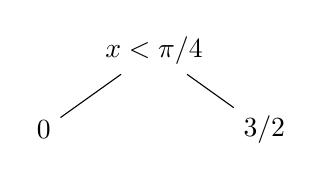
\begin{tikzpicture}
\node (t) at (0,1) {$x<\pi/4$};\node (l) at (-1.4,0) {$0$};\node (r) at (1.4,0) {$3/2$};\draw (t)--(l);\draw (t)--(r);
\end{tikzpicture}\end{center}
Tree B:
\begin{center}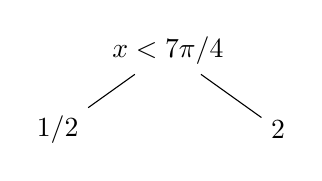
\begin{tikzpicture}
\node (t) at (0,1) {$x<7\pi/4$};\node (l) at (-1.4,0) {$1/2$};\node (r) at (1.4,0) {$2$};\draw (t)--(l);\draw (t)--(r);
\end{tikzpicture}\end{center}
Tree C:
\begin{center}\begin{tikzpicture}
\node (t) at (0,1) {$x<\pi/2$};\node (l) at (-1.4,0) {$0$};\node (r) at (1.4,0) {$1$};\draw (t)--(l);\draw (t)--(r);
\end{tikzpicture}\end{center}

Left branches satisfy the condition; right branches do not.

\par\endgroup

\subsection*{Exercise 4.4 - Combine the predictions}
A \textbf{\textit{forest}} combines predictions from several trees. Use their arithmetic mean:

\[
\hat f_{\mathrm{forest}}(x)=\frac{\hat f_A(x)+\hat f_B(x)+\hat f_C(x)}3.
\]

The leaf predictions are medians; the forest prediction is the mean of the three tree predictions.

\begin{enumerate}
\item
Complete the table at the five original input positions.

\end{enumerate}
\begingroup
\small
\setlength{\tabcolsep}{4pt}
\begin{longtable}{l|l|l|l|l|l|l}
$x$ & Target $f(x)$ & Tree A & Tree B & Tree C & Forest & Absolute forest error \\
\hline
\endfirsthead
$x$ & Target $f(x)$ & Tree A & Tree B & Tree C & Forest & Absolute forest error \\
\hline
\endhead
$0$ & $\phantom{0}$ & $\phantom{0}$ & $\phantom{0}$ & $\phantom{0}$ & $\phantom{0}$ & $\phantom{0}$ \\[3pt]
$\pi/2$ & $\phantom{0}$ & $\phantom{0}$ & $\phantom{0}$ & $\phantom{0}$ & $\phantom{0}$ & $\phantom{0}$ \\[3pt]
$\pi$ & $\phantom{0}$ & $\phantom{0}$ & $\phantom{0}$ & $\phantom{0}$ & $\phantom{0}$ & $\phantom{0}$ \\[3pt]
$3\pi/2$ & $\phantom{0}$ & $\phantom{0}$ & $\phantom{0}$ & $\phantom{0}$ & $\phantom{0}$ & $\phantom{0}$ \\[3pt]
$2\pi$ & $\phantom{0}$ & $\phantom{0}$ & $\phantom{0}$ & $\phantom{0}$ & $\phantom{0}$ & $\phantom{0}$ \\[3pt]
\end{longtable}
\endgroup
\begin{enumerate}
\setcounter{enumi}{1}
\item
Write the forest prediction as a piecewise-constant function. Include every threshold used by any tree.

\item
Sketch the forest prediction.

\item
Calculate the forest's MAE on the original five observations, counting each once. Compare it with the tree from Exercise 4.2.

\end{enumerate}
In a random forest with several input features, a random subset of features can also be considered at each split. Here there is only one feature, so the variation between trees comes from the bootstrap samples.

\begingroup\color{red}

\subsubsection*{Solution 4.4}
\begingroup
\small
\setlength{\tabcolsep}{4pt}
\begin{longtable}{l|l|l|l|l|l|l}
$x$ & Target $f(x)$ & Tree A & Tree B & Tree C & Forest & Absolute forest error \\
\hline
\endfirsthead
$x$ & Target $f(x)$ & Tree A & Tree B & Tree C & Forest & Absolute forest error \\
\hline
\endhead
$0$ & $0$ & $0$ & $\frac{1}{2}$ & $0$ & $\frac{1}{6}$ & $\frac{1}{6}$ \\[1.5pt]
$\pi/2$ & $\frac{3}{2}$ & $\frac{3}{2}$ & $\frac{1}{2}$ & $1$ & $1$ & $\frac{1}{2}$ \\[1.5pt]
$\pi$ & $1$ & $\frac{3}{2}$ & $\frac{1}{2}$ & $1$ & $1$ & $0$ \\[1.5pt]
$3\pi/2$ & $\frac{1}{2}$ & $\frac{3}{2}$ & $\frac{1}{2}$ & $1$ & $1$ & $\frac{1}{2}$ \\[1.5pt]
$2\pi$ & $2$ & $\frac{3}{2}$ & $2$ & $1$ & $\frac{3}{2}$ & $\frac{1}{2}$ \\[1.5pt]
\end{longtable}
\endgroup
Over $[0,2\pi]$,

\[
\hat f_{\mathrm{forest}}(x)=\begin{cases}
1/6,&0\leq x<\pi/4,\\
2/3,&\pi/4\leq x<\pi/2,\\
1,&\pi/2\leq x<7\pi/4,\\
3/2,&7\pi/4\leq x\leq2\pi.
\end{cases}
\]

For the sketch, draw these four horizontal segments. At each threshold,
use the value of the segment to its right.

The MAE on the original five observations is

\[
\mathrm{MAE}_{\mathrm{forest}}=\frac{1/6+1/2+0+1/2+1/2}{5}=\frac13.
\]

This is smaller than the comparison tree's MAE of $2/5$, by $1/15$.


The dashed segments are the forest prediction; the solid curve is the target. At each threshold the filled endpoint belongs to the segment on its right.
\begin{center}
\begin{tikzpicture}[x=3.5cm,y=1.8cm]
\draw[->] (0,0)--(2.2,0) node[right] {$x$};\draw[->] (0,0)--(0,2.4) node[above] {$y$};
\foreach \x/\lab in {0/0,0.5/{\pi/2},1/\pi,1.5/{3\pi/2},2/{2\pi}} {\node[below] at (\x,0) {$\lab$};}
\foreach \y in {0.5,1,1.5,2} {\node[left] at (0,\y) {$\y$};}
\draw[thin,domain=0:2,samples=121] plot (\x,{sin(180*\x)+\x});
\foreach \x/\y in {0/0,0.5/1.5,1/1,1.5/0.5,2/2} {\fill (\x,\y) circle (1.4pt);}
\draw[thick,dashed] (0,0.16666666666666666)--(0.25,0.16666666666666666);\fill (0,0.16666666666666666) circle (1.4pt);
\draw (0.25,0.16666666666666666) circle (1.8pt);
\draw[thick,dashed] (0.25,0.6666666666666666)--(0.5,0.6666666666666666);\fill (0.25,0.6666666666666666) circle (1.4pt);
\draw (0.5,0.6666666666666666) circle (1.8pt);
\draw[thick,dashed] (0.5,1)--(1.75,1);\fill (0.5,1) circle (1.4pt);
\draw (1.75,1) circle (1.8pt);
\draw[thick,dashed] (1.75,1.5)--(2,1.5);\fill (1.75,1.5) circle (1.4pt);
\fill (2,1.5) circle (1.8pt);
\end{tikzpicture}
\end{center}
\par\endgroup

\clearpage
\section*{Part V - Short conceptual questions}
\subsection*{Question 1}
What value does a regression-tree leaf predict when squared error is used?

\begingroup\color{red}

With squared error, a leaf predicts the \textbf{\textit{mean target value}} of the
samples in that leaf.

\par\endgroup

\subsection*{Question 2}
Why is that value the mean?

\begingroup\color{red}

The mean minimizes the sum of squared residuals.

\par\endgroup

\subsection*{Question 3}
What quantity is minimized when choosing a split?

\begingroup\color{red}

A split is chosen to minimize the total error in its child nodes, or
equivalently to maximize the reduction in error.

\par\endgroup

\subsection*{Question 4}
Where do the candidate thresholds come from for a continuous feature?

\begingroup\color{red}

Candidate thresholds can be placed between neighboring distinct
sorted feature values.

\par\endgroup

\subsection*{Question 5}
Why is the prediction of a regression tree piecewise constant?

\begingroup\color{red}

Every leaf predicts a constant, so the overall prediction is
piecewise constant.

\par\endgroup

\subsection*{Question 6}
What is the main effect of increasing tree depth?

\begingroup\color{red}

Increasing depth creates more and smaller regions and usually
reduces training error.

\par\endgroup

\subsection*{Question 7}
Why can a deep tree overfit noisy data?

\begingroup\color{red}

A deep tree can adapt to random fluctuations in the training sample.

\par\endgroup

\subsection*{Question 8}
In a multidimensional input space, what additional choice must the tree make at every split?

\begingroup\color{red}

With several input features, the tree must choose both the
\textbf{\textit{feature}} and the \textbf{\textit{threshold}}.

\par\endgroup

\subsection*{Question 9}
What shape do the regions in the two-dimensional example have when only axis-aligned splits are used?

\begingroup\color{red}

The regions are rectangles, possibly unbounded.

\par\endgroup

\subsection*{Question 10}
Why can bootstrap samples produce different trees from the same original dataset, and how do repeated observations affect the calculation?

\begingroup\color{red}

Bootstrap samples repeat some observations and omit others. This
changes child medians, split errors and sometimes the candidate
thresholds. Every repetition counts separately when sorting targets
and calculating errors.

\par\endgroup

\subsection*{Question 11}
Does averaging the predictions of several regression trees make the forest prediction continuous? Explain.

\begingroup\color{red}

No. A finite average of piecewise-constant tree predictions is still
piecewise constant. Its possible changes occur at the constituent
trees' thresholds. Averaging can reduce jumps, but does not
guarantee continuity; in this example the forest has three nonzero
jumps.

\par\endgroup

\subsection*{Question 12}
Does a smaller training error guarantee better predictions between the training points? Give a short reason.

\begingroup\color{red}

No. The training error measures accuracy only at the observed
positions. A smaller training error does not guarantee more accurate
predictions between them.

\par\endgroup

\subsection*{Key concepts}
\begingroup
\small
\setlength{\tabcolsep}{4pt}
\begin{longtable}{l|l}
Concept & Meaning in this exercise \\
\hline
\endfirsthead
Concept & Meaning in this exercise \\
\hline
\endhead
\textbf{\textit{Regression}} & Predicting a numerical target value. \\[1.5pt]
\textbf{\textit{Observation / feature / target}} & One data point / an input value / the value to be predicted. \\[1.5pt]
\textbf{\textit{Training data}} & Observations used to choose splits and leaf predictions. \\[1.5pt]
\textbf{\textit{Regression tree}} & \shortstack[l]{A sequence of splits dividing the input space into regions with \\ constant predictions.} \\[1.5pt]
\textbf{\textit{Node / root node}} & \shortstack[l]{A stage containing observations / the initial node containing \\ all training observations.} \\[1.5pt]
\textbf{\textit{Parent / child node}} & \shortstack[l]{A node before a split / one of the nodes produced by that \\ split.} \\[1.5pt]
\textbf{\textit{Internal node / leaf}} & \shortstack[l]{A node that splits / a final node assigning a constant \\ prediction.} \\[1.5pt]
\textbf{\textit{Split / threshold}} & A division such as $x<t$ versus $x\geq t$ / its boundary $t$ . \\[1.5pt]
\textbf{\textit{Candidate split}} & \shortstack[l]{A feature-threshold choice tested during training; both \\ children must be non-empty.} \\[1.5pt]
\textbf{\textit{Residual}} & Signed prediction error $r_i=y_i-\hat y_i$ . \\[1.5pt]
\textbf{\textit{Loss}} & A numerical measure of prediction error. \\[1.5pt]
\textbf{\textit{SSE}} & Sum of squared residuals. \\[1.5pt]
\textbf{\textit{MSE / RMSE}} & Mean squared residual / its square root, in target units. \\[1.5pt]
\textbf{\textit{MAE}} & Mean absolute residual. \\[1.5pt]
\textbf{\textit{Mean / median}} & \shortstack[l]{Arithmetic average / middle of the sorted values, \\ conventionally averaging the middle pair for even sample size.} \\[1.5pt]
\textbf{\textit{Error reduction}} & Parent SSE minus the sum of child SSEs. \\[1.5pt]
\textbf{\textit{Tree depth}} & Maximum number of splits on a root-to-leaf path. \\[1.5pt]
\textbf{\textit{Piecewise-constant prediction}} & A prediction constant inside each leaf region. \\[1.5pt]
\textbf{\textit{Training error}} & Prediction error on the observations used to build the model. \\[1.5pt]
\textbf{\textit{Noise / overfitting}} & \shortstack[l]{Random target variation / fitting sample-specific details in a \\ way that harms prediction on new data.} \\[1.5pt]
\textbf{\textit{Feature space}} & The space of possible combinations of input features. \\[1.5pt]
\textbf{\textit{Axis-aligned split}} & A split testing only one feature. \\[1.5pt]
\textbf{\textit{Bootstrap sample}} & \shortstack[l]{A sample drawn with replacement; observations may repeat or be \\ absent. Here each sample has five draws.} \\[1.5pt]
\textbf{\textit{Forest}} & \shortstack[l]{A collection of trees whose predictions are combined; here by \\ their arithmetic mean.} \\[1.5pt]
\textbf{\textit{Total absolute split error}} & \shortstack[l]{$S=N_L\mathrm{MAE}_L+N_R\mathrm{MAE}_R$ , counting each \\ observation in its child.} \\[1.5pt]
\end{longtable}
\endgroup

\end{document}
